\clearpage
\section{プログラミングの準備をしよう}
\subsection{ファイルって何だろう}

皆さんが使っているRaspberry Piは、パソコンと同じように内部のきおく装置に
「ファイル」「フォルダ」という単位で情報が記録されています。
\begin{description}
  \item[ファイル]\mbox{}\\
  データをひとまとまりにして、名前を付けたもの
  \item[フォルダ]\mbox{}\\
  ファイルをひとまとまりにして、名前を付けたもの
\end{description}
  

以前に使ったフォルダを覚えていますか?上にあるバーのフォルダアイコンからウインドウを開いてみましょう。

\begin{figure}[H]
  \begin{center}
    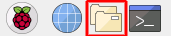
\includegraphics[keepaspectratio,width=5.898cm,height=1.242cm]{images/chap02/text02-img001.png}
    \caption{フォルダウインドウを開くアイコン}
  \end{center}
  \label{fig:folder_icon}
\end{figure}

これから作業で使うファイルをコピーしてもらいます。
皆さんは、「/home/ユーザー名」のフォルダに、第1回で使うフォルダ「01」をコピーしているはずです。
今日は、「02」フォルダをコピーしてから始めます。
まず、「/usr/local/share/ome」という場所を開いてみましょう。
どこにあるか探すことができますか?
わからない時は、TAや先生に聞いてみましょう。

\begin{figure}[H]
  \begin{center}
    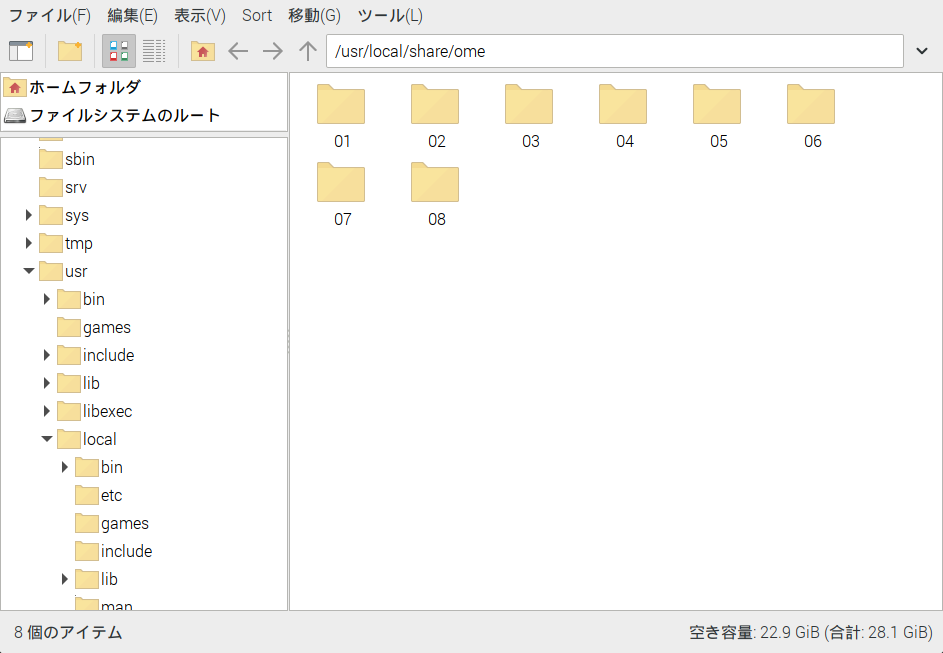
\includegraphics[keepaspectratio,width=11.232cm,height=8.424cm]{images/chap02/s_ome02a.png}
    \caption{/usr/local/share/ome フォルダ}
  \end{center}
  \label{fig:folder_ome}
\end{figure}

\noindent
この中に、「02」という名前のフォルダがあります。
これから、この「02」というフォルダを自分の作業フォルダにコピーします。
「02」という名前のフォルダ上でマウスの右クリックを押して「コピー」を選んでください。

\begin{figure}[H]
  \begin{center}
    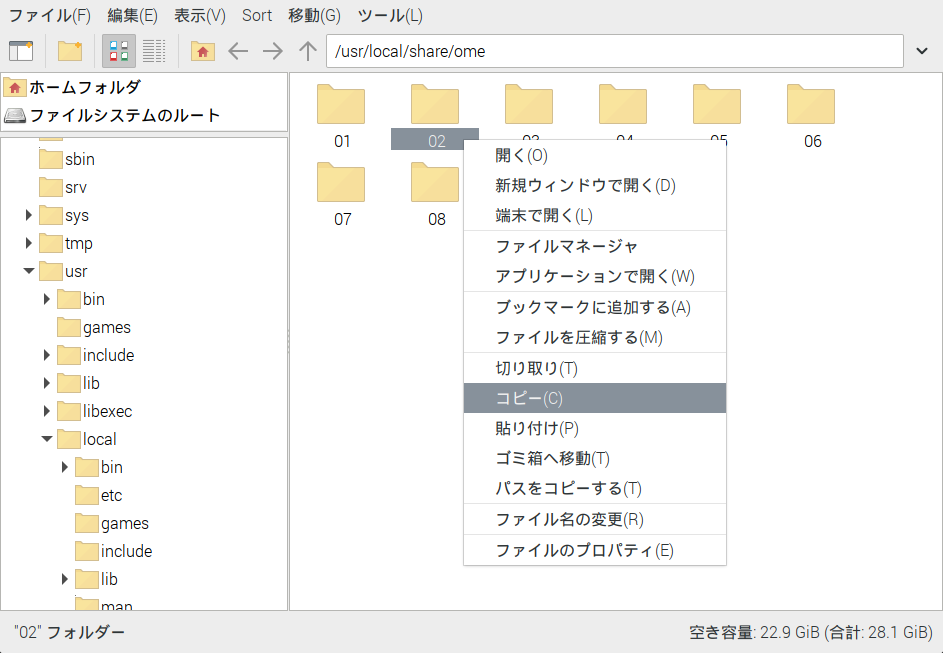
\includegraphics[keepaspectratio,width=11.232cm,height=8.424cm]{images/chap02/s_ome02b.png}
    \caption{02フォルダでコピーを選ぶところ}
  \end{center}
  \label{fig:folder_02copy}
\end{figure}

\noindent
コピーを選ぶだけでは何も起こりません。この後、コピーしたい場所を選びます。
コピー先の場所は、「/home/ユーザー名」のフォルダになります。
たとえば、ユーザー名が「ome」だった場合は、「/home/ome」という場所にコピーします。
コピー先の場所を開いたら、何もない場所でマウスの右クリックを押して「貼り付け」を選んでください。

\begin{figure}[H]
  \begin{center}
    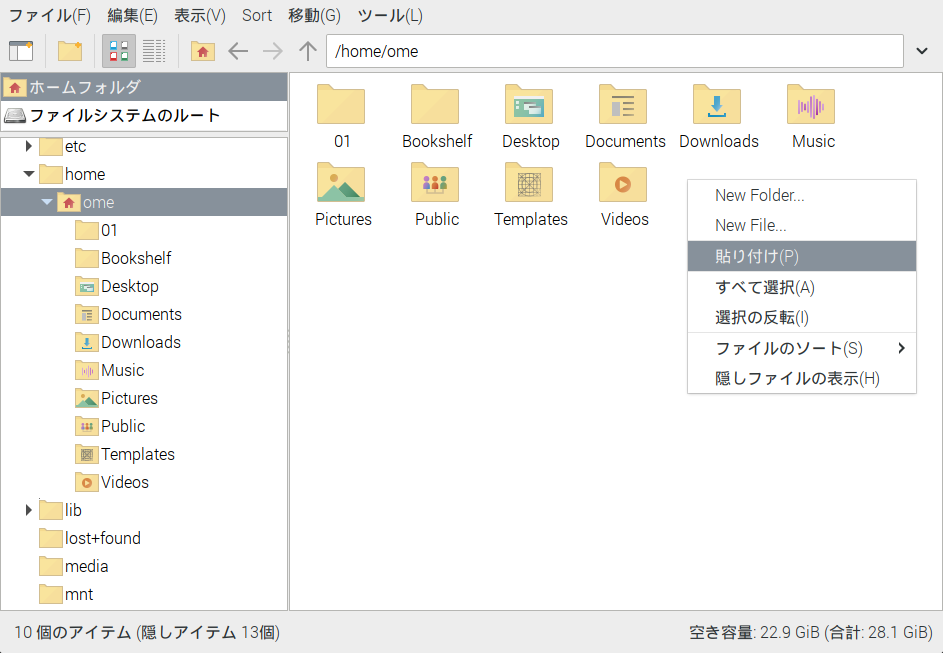
\includegraphics[keepaspectratio,width=11.232cm,height=8.424cm]{images/chap02/s_ome02c.png}
    \caption{02フォルダで貼り付けを選ぶところ}
  \end{center}
  \label{fig:folder_02paste}
\end{figure}

\noindent
これで先ほどの「/usr/local/share/ome/02」フォルダが、「/home/ユーザー名/02」にコピーされます。
ファイルのコピー、移動、削除などの方法を、よく覚えておきましょう。
ファイルには、画像や文章、音声や動画など、さまざまなデータが入っています。
これから皆さんが作業で使うファイルは、「/home/ユーザー名/02」という場所に置かれています。
ファイルの中身が何なのか、自分が作ったファイルかどうかを知っておいてください。

\begin{figure}[H]
  \begin{center}
    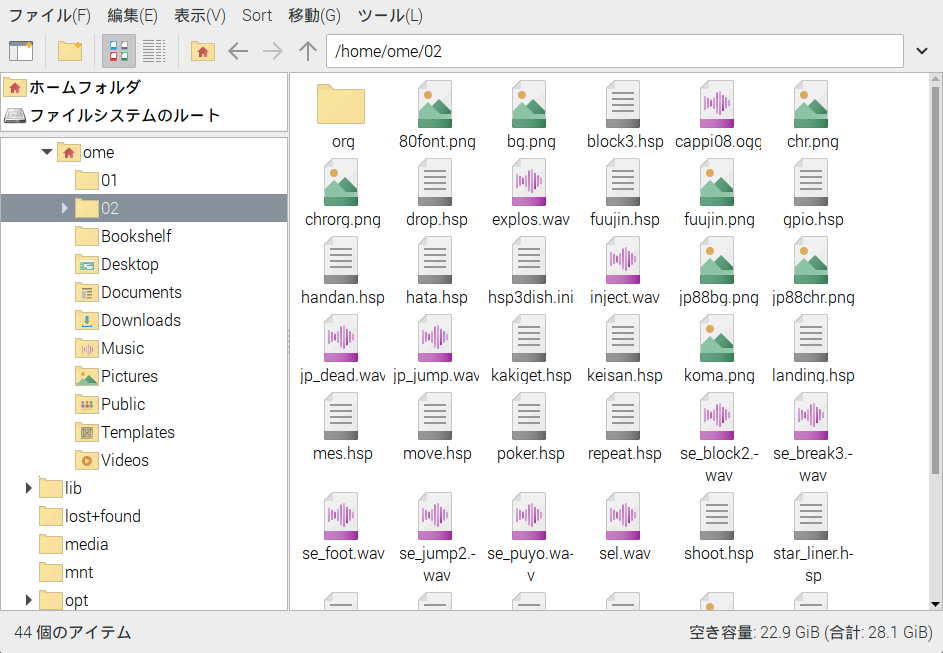
\includegraphics[keepaspectratio,width=11.232cm,height=8.424cm]{images/chap02/s_ome02d.png}
    \caption{02フォルダを開いたところ}
  \end{center}
  \label{fig:folder_02open}
\end{figure}
\clearpage


\subsection{ターミナルの使い方}
これから、Raspberry Piを使って色々なゲームを作ったり、改造したりといった作業をします。
以下の2つに注意しながら、作業を進めていきましょう。

\begin{itemize}
  \item 自分が作ったファイル以外は削除や移動しないようにしましょう
  \item ファイルやフォルダはわかりやすい場所に作りましょう
\end{itemize}

ターミナルの使い方を覚えておきましょう。
ターミナル(コマンドライン)は、キーボードの入力だけでコンピューターをそうさするためのものです。

\begin{figure}[H]
  \begin{center}
    
\includegraphics[keepaspectratio,width=7.303cm,height=1.15cm]{images/chap02/text02-img003.png}
    \caption{ターミナル起動アイコン}
  \end{center}
  \label{fig:terminal_icon}
\end{figure}

ターミナル起動アイコンを選択すると、ターミナル画面のウインドウが開きます。

\begin{figure}[H]
  \begin{center}
    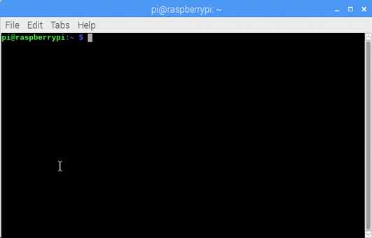
\includegraphics[keepaspectratio,width=9.472cm,height=6.061cm]{images/chap02/text02-img004.png}
    \caption{ターミナル画面}
  \end{center}
  \label{fig:terminal_display}
\end{figure}

\noindent
黒い画面が出てきました。ちょっと難しそうですね。

ターミナルの使い方を覚えておくと、キーボードだけで手早くコンピューターを扱うことができるようになります。
すべての人が必ず使うものではありませんが、とても便利に使うことができるので、少しずつ使って慣れるようにしていきましょう。

\noindent
たとえば、

\vspace{1em}
\ \ \ \ ls [Enter]
\vspace{1em}
  
\noindent
を入力するとファイルの一覧が出てきます。

\begin{figure}[H]
  \begin{center}
    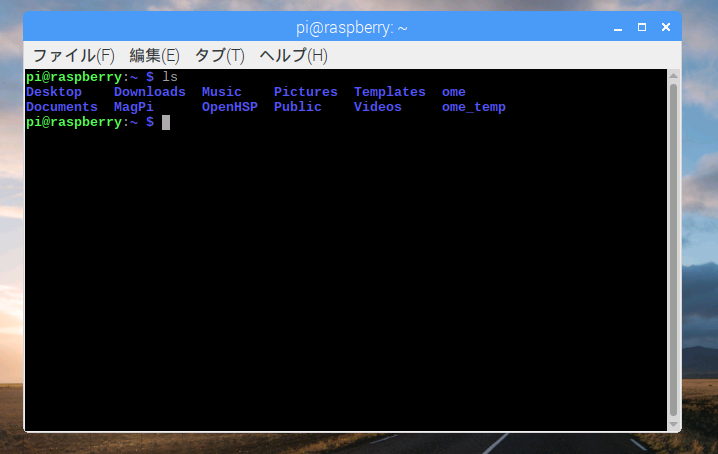
\includegraphics[width=9.71cm,height=6.138cm]{images/chap02/text02-img005.png}
    \caption{lsコマンドを入力した画面}
  \end{center}
  \label{fig:terminal_ls}
\end{figure}

今回、プログラミングやターミナルなど、キーボードをたくさん使う機会があります。
最初は難しいかもしれませんが、思ったように文字を打つことができるよう、練習をして覚えていきましょう。

キーボードは乱暴に扱わない方がいいですが、間違ったボタンを押したからと言ってコンピューターがこわれることはありません。
ですから、間違えることを心配せずに、どんどん自分からキーボードをそうさして、使い方に慣れるよう心掛けてください。

% 
% 
% 
\subsection{プログラミングって何だろう}

皆さんには、プログラミングを初めてもらいます。
プログラミングというのは、プログラムを作ることです。
さて、そもそもプログラムって何でしょう?
パソコンの上で動いている、ワープロソフトやペイントソフト、ゲームなどもみんなまとめて「プログラム」と呼んでいます。

スマホのアプリもプログラムと同じです。ゲーム機のゲームソフトもプログラムです。
「プログラム」というのは自分が考えた通りに動いてくれる予定表のようなものです。
たとえば、学校の授業や運動会にもプログラム(予定表)があり、どんな順番で何をするか決められています。
ビデオレコーダーがテレビ番組を決められた時間に勝手に録画してくれるのもプログラムです。パソコンで動くプログラムは、もっともっと色々な仕事をすばやくこなすことができるものなのです。

\begin{description}
  \item[電化製品]\mbox{}\\
  家庭で使われている電化製品にも、コンピューターとプログラムが使われています。今では、電気を使うほとんどの機器が、プログラムによって動いています。
  \item[ゲーム機]\mbox{}\\
  現在は様々なハードでゲームが遊べるようになっていますが、ビデオゲームは色々な進化をたどってきました。今では、とても高度なコンピューターが使われています。
  \item[ロボットや人工知能]\mbox{}\\
  これから大きく発展する分野が、ロボットや人工知能です。これらは、コンピューターと高度なプログラムを組み合わせて作られています。
  まだ、簡単なことしかできないロボットが、将来は人間と同じ能力を持って仕事をしているかもしれません。
\end{description}

\begin{figure}[H]
  \begin{center}
    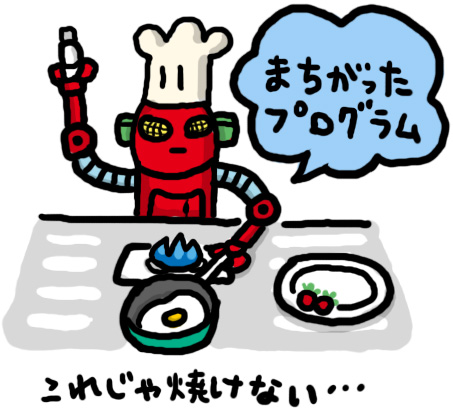
\includegraphics[width=8.031cm,height=7.304cm]{images/chap02/text02-img006.jpg}
    % \caption{robot}
  \end{center}
  \label{fig:robot}
\end{figure}
\clearpage

% 
% 
% 
\subsection{HSPに触れてみよう}

それでは、さっそくプログラム作りを始めてみましょう。
プログラムを作ったり、打ち込んだりすることをプログラミングといいます。
これから、やることの内容はつぎの通りです。

\begin{itemize}
  \item \textbf{プログラムの呼び出し方と動かし方を覚える}
  \item \textbf{センサーボードを使って仕組みを覚える}
  \item \textbf{プログラムを自分の手で実際に打ち込んでみること}
  \item \textbf{ゲームを改造して自分だけのオリジナルゲームにすること}
\end{itemize}

プログラムを覚えたら、何ができるのか?
そして、プログラムを覚えておくと将来どんないいことがあるのか?
皆さんもプログラムの世界について学んでいきましょう。

今回みなさんに使ってもらうのは「ホットスーププロセッサ ( Hot Soup Processor )」、
りゃくして「HSP(エッチ・エス・ピー)」と呼ばれているツールです。
ゲームを作るのに向いているだけでなく、小中学生にも使えるくらい簡単で、参考になる本もいっぱい出ています。

左上のRaspberry Piメニューの「プログラミング」項目に、
「HSP Script Editor」(HSPスクリプトエディタ)という項目があるはずです。
メニューを開いて確認(かくにん)してみましょう。

\begin{figure}[H]
  \begin{center}
    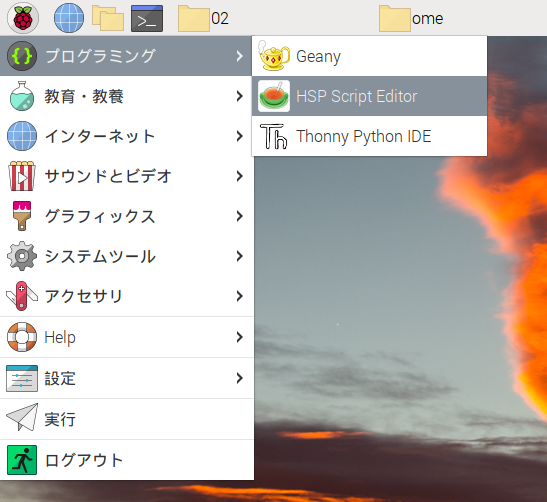
\includegraphics[keepaspectratio,width=7.31cm,height=6.562cm]{images/chap02/s_hspmenu.png}
    \caption{プログラミング項目のメニュー}
  \end{center}
  \label{fig:hsp_menu}
\end{figure}

「HSP Script Editor」のアイコンをクリックして起動させてみましょう。
Raspberry Piメニューからでも、ターミナルから「hsed」と打ち込んでも起動させることができるので
覚えておきましょう。

\begin{figure}[H]
  \begin{center}
    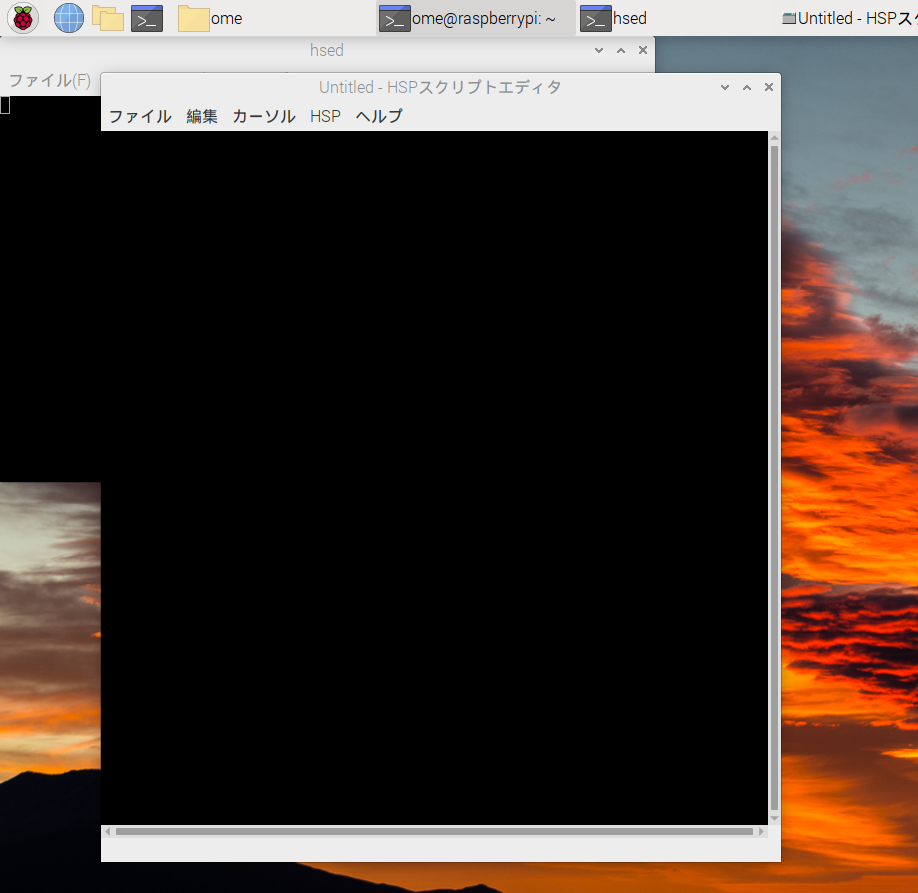
\includegraphics[keepaspectratio,width=7.31cm,height=6.562cm]{images/chap02/s_hsed.png}
    \caption{HSPスクリプトエディタを起動したところ}
  \end{center}
  \label{fig:hsed_start}
\end{figure}

「HSPスクリプトエディタ」は、テキストエディタ(MousePad)と同じように好きな文字を打ち込むことができます。
文字を直したり、カーソルを好きな場所に移動したりする方法がわからない人は、近くの先生に聞いてみてください。

実際にできあがっているプログラムを見てみましょう。
ファイル→「開く」メニューから 「/home/ユーザー名/02」フォルダの中にある「shoot.hsp」を読み込んでください。
作業は、すべて「/home/ユーザー名/02」フォルダで行います。
見つからない場合は、まわりの友達か、近くの先生に聞いてみてください。

\begin{figure}[H]
  \begin{center}
    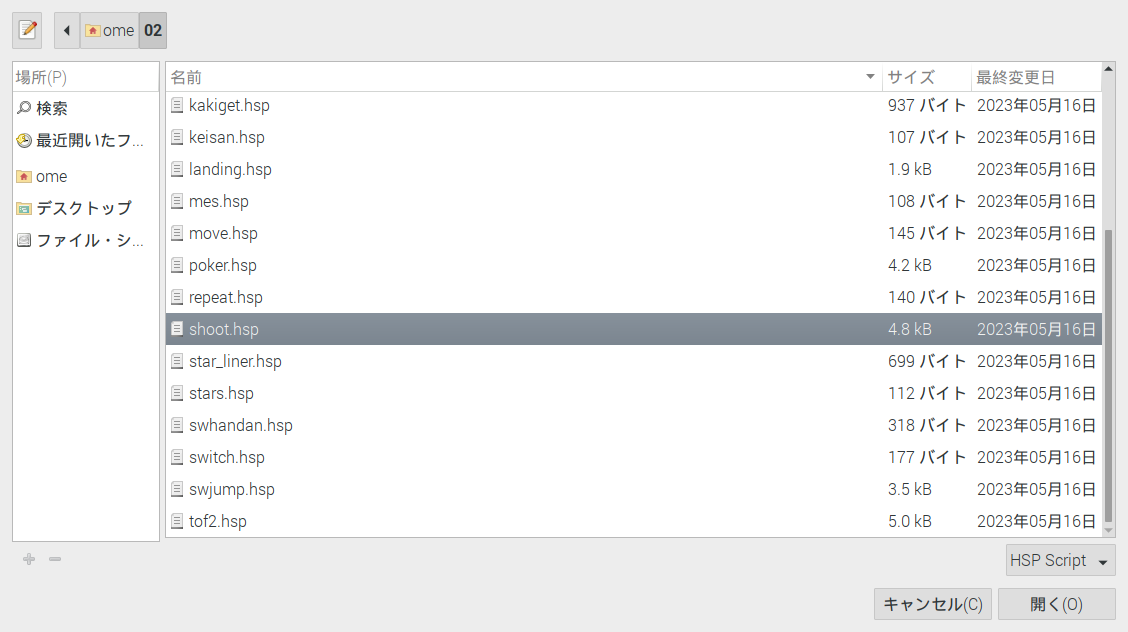
\includegraphics[keepaspectratio,width=7.31cm,height=6.562cm]{images/chap02/s_openfolder.png}
    \caption{フォルダから読み込む画面}
  \end{center}
  \label{fig:hsed_openfolder}
\end{figure}

だらだらと長い文字が読み込まれましたか?
今は意味がわからなくても大丈夫です。

まずは、[F5]キーを押して動かしてみましょう。
[F5]キーを押すと読み込まれたスクリプトをもとにプログラムがうごきだします。
\clearpage

% 
% 
% 
\subsection{シューティングゲームの遊び方}

\begin{enumerate}
  \item タイトル画面で[Enter]キーを押すとゲームがスタートします
  \item カーソルキーで上下左右に移動、ミサイルは自動発射です
  \item 敵や弾に当たるとゲームオーバーになってしまいます
\end{enumerate}

\begin{figure}[H]
  \begin{center}
    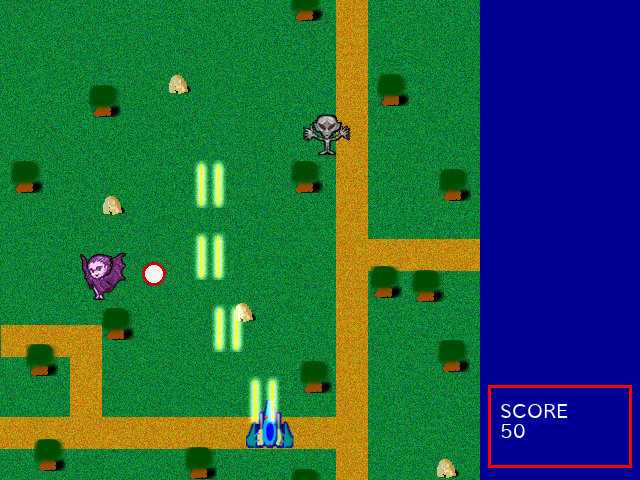
\includegraphics[keepaspectratio,width=7.31cm,height=6.562cm]{images/chap02/s_shoot.png}
    \caption{シューティングゲームの画面}
  \end{center}
  \label{fig:hsp_shoot}
\end{figure}

ゲームを遊び終わったらウインドウ右上の「×」を押してウィンドウを閉じましょう

\begin{figure}[H]
  \begin{center}
    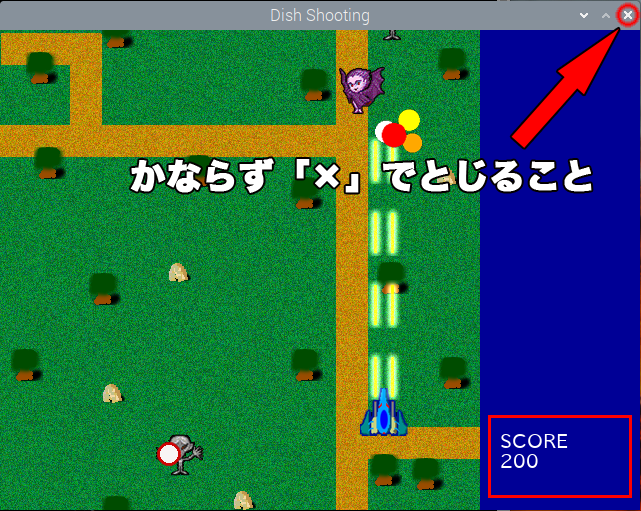
\includegraphics[keepaspectratio,width=7.31cm,height=6.562cm]{images/chap02/s_shoot2.png}
    \caption{ウインドウを閉じるボタン}
  \end{center}
  \label{fig:hsp_shoot2}
\end{figure}

このようにスクリプトがあればゲームを動かすことができます。
ゲームが終わったら、かならず「×」ボタンを押してエディタの画面に戻ってください。
「×」ボタンを押さないと、スクリプトエディタのそうさに戻ることができません。

さて、このスクリプトエディタに表示されている長い文章のことを「スクリプト」と呼びます。
「プログラム」は、できあがったもの全体を指してまぎらわしいので、
プログラミングで打ち込むための言葉は「スクリプト」と呼ぶようにしますので覚えておいてください。

HSPスクリプトエディタは、打ち込まれたスクリプトを[F5]キーで実行する機能、
そのスクリプトを.hspファイルとして保存したり読み込んだりする機能があります。
実行された時には、新しいウインドウに表示され、右上の[×]ボタンを押すことで、元の編集画面に戻ります。

\begin{figure}[H]
  \begin{center}
    
\includegraphics[width=15.533cm,height=4.86cm]{images/chap02/text02-img013.png}
    % \caption{shoot3}
  \end{center}
  \label{fig:hsp_shoot3}
\end{figure}

HSPスクリプトエディタの基本的な使い方をよく覚えておきましょう。
スクリプトを書けるようになると、画面の絵や音、そしてハードウェアなど様々なデバイスを組み合わせて、
あなたの考えたプログラムを作ることができるようになります。
\clearpage

% 
% 
% 
\subsection{例題に挑戦しよう}

ここまで終わってしまった人は、以下の例題にも挑戦してみよう。

\begin{itemize}
  \item ターミナルからHSPスクリプトエディタを起動する
  \item ドロップパズル(drop)を読み込んで動かす
  \item ブロック崩し(block3)を読み込んで動かす
  \item その他のゲームでラズパイに親しむ
\end{itemize}

\noindent
例題の考え方がわからない時は、近くのTAか先生に聞いてください。
わからない所は、そのままにせず、必ず答えを見つけてから先に進みましょう。
\clearpage

% 
% 
% 
\subsection{例題1 HSPスクリプトエディタをターミナルから起動する}

\subsubsection*{考え方}

ターミナルからHSPスクリプトエディタを起動してみましょう。
HSPスクリプトエディタを起動するためのコマンドは、「hsed」です。

\subsubsection*{例題1 答え}

プログラムを打ち込むためには、「HSPスクリプトエディタ」というツールを使うことを覚えました。
Raspberry Piメニューにある「HSP ScriptEditor」のアイコンをクリックして起動させることができるほか、
ターミナルからhsedコマンドで直接起動させることもできます。

ターミナル起動アイコンを選択すると、ターミナル画面のウインドウが開きます。

\begin{figure}[H]
  \begin{center}
    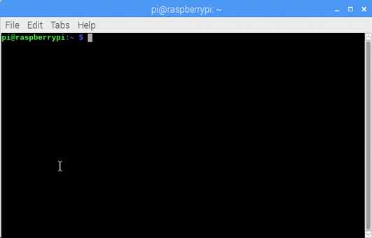
\includegraphics[keepaspectratio,width=8.52cm,height=5.45cm]{images/chap02/text02-img004.png}
    \caption{ターミナル画面}
  \end{center}
  \label{fig:terminal}
\end{figure}

ターミナルの画面で

\vspace{1em}
\ \ \ \ hsed [Enter]
\vspace{1em}

\noindent
と入力しましょう。
HSPスクリプトエディタが起動することを確認(かくにん)してください。
\clearpage

% 
% 
% 
\subsection{例題2 ドロップパズル(drop)を読み込んで動かす}

\subsubsection*{考え方}

HSPスクリプトエディタからスクリプト(プログラム)を読み込む方法と、実行する方法を思い出してみてください。
それでは、HSPスクリプトエディタからドロップパズル(drop.hsp)を読み込んで遊んでみましょう。
ドロップパズル(drop.hsp)は、/home/ユーザー名/02のフォルダにあります。

\subsubsection*{例題2 答え}

HSPスクリプトエディタの基本的な使い方をよく覚えておきましょう。

\begin{figure}[H]
  \begin{center}
    
\includegraphics[keepaspectratio,width=15.533cm,height=4.86cm]{images/chap02/text02-img013.png}
    % \caption{hsed}
  \end{center}
  \label{fig:hsed_chart}
\end{figure}

\noindent
このように、HSPスクリプトエディタは、打ち込まれたスクリプトを[F5]キーで実行する機能、
そのスクリプトを.hspファイルとして保存したり読み込んだりする機能があります。
実行した後には、ウインドウの「×」ボタンを押して元の画面に戻ります。

ファイル→「開く」メニューから/home/ユーザー名/02のフォルダに移動してから、「drop.hsp」を読み込んでみましょう。

\begin{figure}[H]
  \begin{center}
    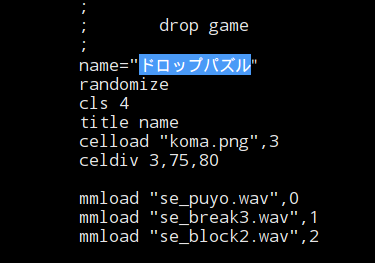
\includegraphics[keepaspectratio,width=9.049cm,height=6.346cm]{images/chap02/text02-img014.png}
    \caption{ドロップパズルのスクリプト}
  \end{center}
  \label{fig:drop_script}
\end{figure}

\noindent
読み込まれたら、[F5]キーで実行します。

\begin{figure}[H]
  \begin{center}
    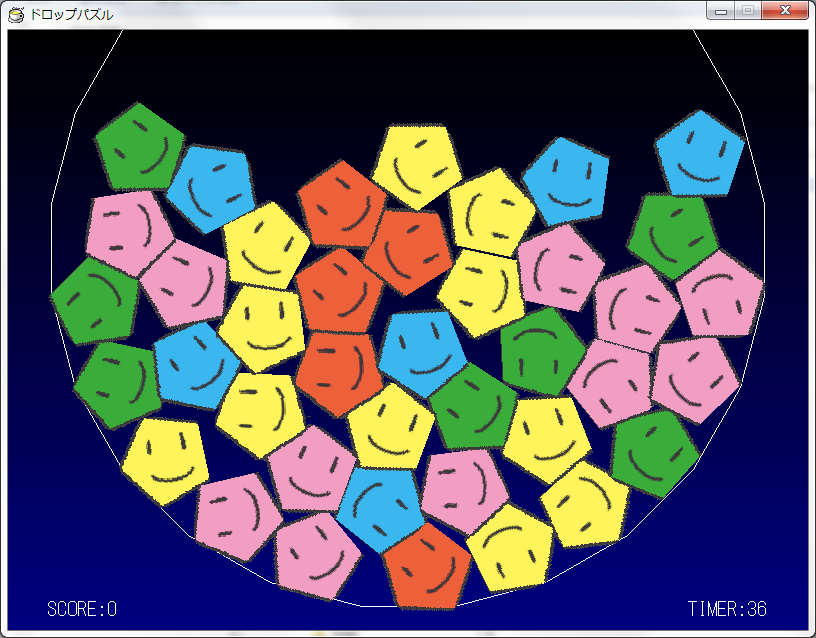
\includegraphics[keepaspectratio,width=9.049cm,height=6.346cm]{images/chap02/text02-img015.png}
    \caption{ドロップパズルゲームの画面}
  \end{center}
  \label{fig:drop_display}
\end{figure}

ドロップパズルは、上から落ちてくる5角形のパネルをうまく消していくゲームです。
パネルの上にマウスカーソルを合わせて、ボタンを押しながら同じ色のパネルをなぞってください。
すると、同じ色のパネルが消えて、新しいパネルが上から降ってきます。
一度に同じ色のパネルをたくさん消すと、高いスコアがもらえます。
時間内にできるだけ高いスコアを出せるように頑張ってください。

ゲームを終了する時は、ウインドウの「×」ボタンを押してください。
\clearpage

% 
% 
% 
\subsection{例題3 ブロック崩し(block3)を読み込んで動かす}

\subsubsection*{考え方}

/home/ユーザー名/02のフォルダにある他のスクリプトを実行してみましょう。
「block3.hsp」は、ブロック崩しゲームのスクリプトです。
ドロップパズルと同じように読み込んで動かしてみましょう。

\subsubsection*{例題3 答え}

ファイル→「開く」メニューから/home/ユーザー名/02のフォルダに移動してから、「block3.hsp」を読み込んでみましょう。
読み込まれたら、[F5]キーで実行します。

マウスをうまく動かしてラケットをそうさします。ボールを打ち返してブロックを崩してください。
ボールが下まで落ちてしまうとアウトです。

\begin{figure}[H]
  \begin{center}
    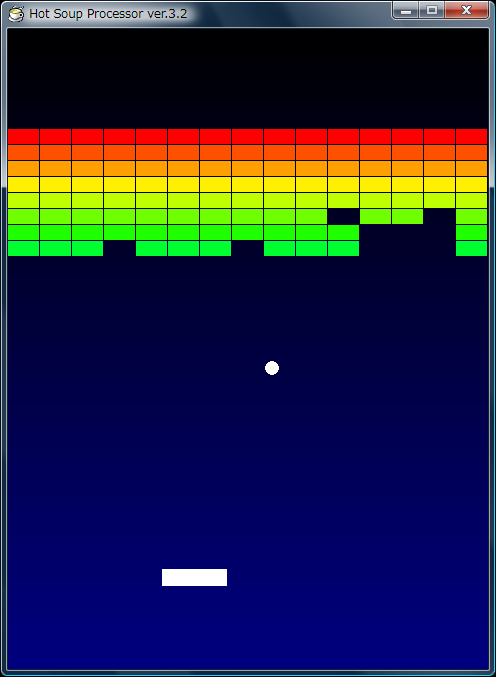
\includegraphics[keepaspectratio,width=9.049cm,height=6.346cm]{images/chap02/text02-img016.png}
    \caption{ブロック崩しの画面}
  \end{center}
  \label{fig:block_display}
\end{figure}

ゲームを終了する時は、ウインドウの「×」ボタンを押してください。
\clearpage

% 
% 
% 
\subsection{例題4 重力ゲーム(tof2)を読み込んで動かす}

\subsubsection*{考え方}

/home/ユーザー名/02のフォルダにある他のスクリプトを実行してみましょう。
「tof2.hsp」は、重力ゲームのスクリプトです。
ドロップパズルと同じように読み込んで動かしてみましょう。

\begin{figure}[H]
  \begin{center}
    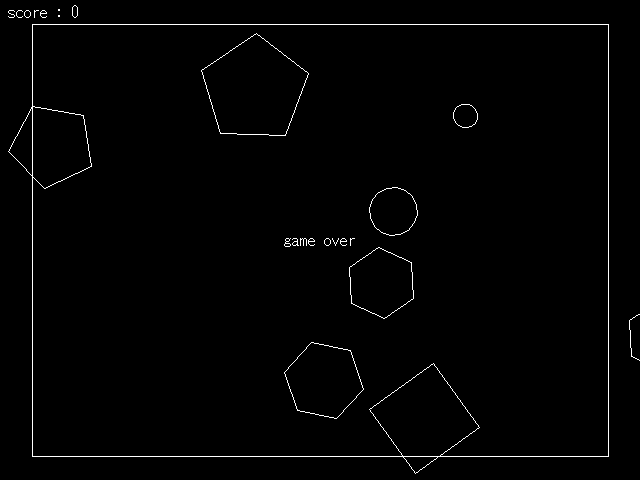
\includegraphics[keepaspectratio,width=8.467cm,height=7.17cm]{images/chap02/s_tof2.png}
    \caption{tof2の画面}
  \end{center}
  \label{fig:tof2}
\end{figure}

ゲームを終了する時は、ウインドウの「×」ボタンを押してください。

\subsubsection*{例題4 答え}

カーソルキーで大きな円をうまく動かして小さい円をバウンドさせます。
小さい円で敵を攻撃することができます。できるだけ多くの敵を倒してください。

ゲームを終了する時は、ウインドウの「×」ボタンを押してください。











% \clearpage
% % \chapter{ゲームを\ruby{改造}{かい|ぞう}してみよう}
% \section{今回の授業}
% \subsection{目標}
% \begin{itemize}
%   \item プログラムについて知ろう
%   \item センサーとゲームで遊んでみよう
% \end{itemize}

% \subsection{授業内容}
% \begin{enumerate}
%   \item プログラミングの準備をしよう
%   \item ゲームで遊んでみよう
%   \item センサーボードを使ってみよう
%   \item プログラムを改造してみよう
% \end{enumerate}

% \subsection{注意点}
% \begin{itemize}
%   \item 授業の合間のきゅうけいでは、遠くのものをながめたりして目を休めましょう
%   \item 水分ほきゅうはこまめにしましょう
%   \item 先生が説明中は先生の話を聞きましょう
%   \item わからないことがあったらTAの先生方にすぐ聞きましょう
% \end{itemize}

% \subsection{ラズベリーパイを使うときの注意}
% \begin{itemize}
%   \item 水などぬれているものをラズベリーパイ本体につけないようにしましょう
%   \item ラズベリーパイをはじめコンピュータなどは熱に弱いのですごく暑い部屋では使わないようにしましょう
%   \item ラズベリーパイなどは静電気によわいので注意しましょう
%   \item ラズベリーパイをらんぼうに扱うのはやめましょう
% \end{itemize}
% \clearpage








% \begin{lstlisting}[caption=Tabの例2, label=Tab2]
%   <#green#pi@raspberrypi#>:<#blue#~ $#> cat ~/P
%   <#green#pi@raspberrypi#>:<#blue#~ $#> cat ~/Pictures	<--Tabを打つと出てくる
% \end{lstlisting}


% \begin{description}
% \item[コマンド\textvisiblespace オプション\textvisiblespace \ruby{引数}{ひき|すう}1\textvisiblespace 
% \ruby{引数}{ひき|すう}2]\mbox{}\\
%  コマンドは動作、引数はそうさのたいしょうです。
%  コマンドの最後にEnterキー(エンターキー)を\ruby{押}{お}して、
%  コンピュータにコマンドを送ります。
%  EnterキーはReturn(リターン)キーと\ruby{呼}{よ}ぶこともあります。
% \end{description}



% \begin{lstlisting}[caption=pwdコマンドの例,label=pwdtest]
% <#green#pi@raspberrypi#>:<#blue#~ $#> pwd
% /home/pi   <-- カレントディレクトリが表示されます
% <#green#pi@raspberrypi#>:<#blue#~ $#>
% \end{lstlisting}

% \begin{tcolorbox}[title=\useOmetoi]
% \begin{enumerate}
% \addquiz{\ruby{実際}{じっ|さい}にpwdを使って、カレントディレクトリが\ruby{表示}{ひょう|じ}されることを確かめましょう。
%         表示されたカレントディレクトリを書いてください。}
% \end{enumerate}
% \end{tcolorbox}

% \subsection{ディレクトリの中を見てみよう}
% \begin{description}
% \item[\texttt{ls}\textvisiblespace \texttt{-F}\textvisiblespace ディレクトリ]\mbox{}\\
% ディレクトリの中のファイルやディレクトリが表示されます。
% ファイルはピンクの文字、ディレクトリは青い文字になっています。
% Fは大文字なので注意してください。
% \end{description}

% %//terminal[lsF-test][ls -F コマンドの例]{
% \begin{minipage}{\linewidth}
% \begin{lstlisting}[caption=ls -F コマンドの例。ファイルやディレクトリが表示されます,label=lsFtest]
% <#green#pi@raspberrypi#>:<#blue#~ $#> ls -F
% <#blue#01  03         Desktop    Downloads  Pictures  Templates
% 02  Bookshelf  Documents  Music      Public    Videos#>
% <#green#pi@raspberrypi#>:<#blue#~ $#>
% \end{lstlisting}
% \end{minipage}


% ディレクトリの中にあるファイルは人によってちがいます。
% \begin{lstlisting}[caption=ls -F Pictures/コマンドの例,label=lsFPicttest]
% <#green#pi@raspberrypi#>:<#blue#~ $#> ls -F Pictures
% <#magenta#2019-07-08-145604_1366X768_scrot.png  2019-07-08-150326_1366X768_scrot.png  
% 2019-07-08-150313_1366X768_scrot.png  2019-07-08-150348_1366X768_scrot.png  
% 2019-07-08-150323_1366X768_scrot.png  2019-07-08-150356_1366X768_scrot.png  #>
% <#green#pi@raspberrypi#>:<#blue#~ $#> 
% \end{lstlisting}

% \begin{tcolorbox}[title=\useOmetoi]
% \begin{enumerate}
% \addquiz{\texttt{ls}\textvisiblespace \texttt{-F}と入力して出てきたファイルとディレクトリの名前を1つずつ書きましょう。Fは大文字です。}
% \addquiz{\texttt{ls}\textvisiblespace \texttt{-F}\textvisiblespace Pictures/ と入力して出てきたファイルかディレクトリの名前を1つ書きましょう。}
% \end{enumerate}
% \end{tcolorbox}


% \begin{table}[H]
%   \begin{center}
%     \caption[tab:files]{ファイルの種類}
%     \begin{tabular}{|c|c|c|} \hline
%     \begin{minipage}{0.3\hsize}
%       \begin{center}
%         \includesvg[width=\linewidth]{images/chap03/oto.svg}
%       \end{center}  
%     \end{minipage} & 
%     \begin{minipage}{0.3\hsize}
%       \begin{center}
%         \includesvg[width=\linewidth]{images/chap03/image.svg}
%       \end{center}
%     \end{minipage} &
%     \begin{minipage}{0.3\hsize}
%       \begin{center}
%         \includesvg[width=\linewidth]{images/chap03/douga.svg}
%       \end{center} 
%     \end{minipage} \\ \hline
%     oto.mp3 & gazou.jpg & douga.mp4 \\ \hline
%   \end{tabular}
%  \end{center}
% \end{table}


% \begin{figure}[H]
%     \begin{minipage}{0.4\hsize}
%         \includesvg[width=\hsize]{images/chap03/directory_arc.svg}
%     \end{minipage}
%     \begin{minipage}{0.6\hsize}
%         \begin{itemize}
%         \item /は一番上のディレクトリから見ると/
%         \item /はカレントディレクトリが/のとき./
%         \item /はカレントディレクトリがhomeのとき../
%         \item /はカレントディレクトリがpiのとき../../
%         \item homeは一番上のディレクトリから見ると/home
%         \item homeはカレントディレクトリが/のとき./home
%         \item homeはカレントディレクトリがhomeのとき./
%         \item homeはカレントディレクトリがpiのとき../
%         \item piは一番上のディレクトリから見ると/home/pi
%         \item piはカレントディレクトリが/のとき./home/pi
%         \item piはカレントディレクトリがhomeのとき./pi
%         \item piはカレントディレクトリがpiのとき./
%         \end{itemize}
%     \end{minipage}
%     \caption{フォルダ間の関係をパスで説明する}
%     \label{fig:folder-path}
% \end{figure}

